\documentclass[12pt]{article}

\newif\ifpdf
\ifx\pdfoutput\undefined
\pdffalse % not running PDFLaTeX
\else
\pdfoutput=1 % running PDFLaTeX
\pdftrue
\fi

\ifpdf
\usepackage[pdftex]{graphicx}
\else
\usepackage{graphicx}
\fi

%\usepackage[osf]{gtamachoefler}

% Added by bcarey
% Bibliography support
\usepackage{lscape}
\usepackage[super,comma,sort]{natbib} 
%\usepackage[linux]{vpe}
%\vpesetup{noref}
%define citation punctuation style
\bibpunct[, ]{(}{)}{;}{a}{,}{,}

% Allow less text and more figure on page
\renewcommand{\topfraction}{0.90}
\renewcommand{\bottomfraction}{0.90}
\renewcommand{\textfraction}{0.1}
\renewcommand{\floatpagefraction}{0.90}

% end additions by bcarey


%\usepackage{times}
\usepackage{fourier}
\usepackage{sectsty,hangcaption}
\usepackage{amsmath,amsbsy,amssymb}
%\usepackage{deflist}
\usepackage{fancyhdr}
\usepackage{tabularx}
\usepackage{verbatim}
\usepackage{moreverb}
\usepackage{float}
\usepackage{fancybox}
\usepackage{graphicx}
\usepackage{longtable}
\usepackage{wrapfig}
\usepackage{booktabs}
\usepackage{comment}
%\usepackage{subfigure}

%must be last package
%\usepackage{hyperref}
\usepackage[debug=false, colorlinks=true, pdfstartview=FitV, linkcolor=blue, citecolor=blue, urlcolor=blue]{hyperref}

%\usepackage{toc_entr}
\textwidth 6.5in
\textheight 9.in
%\topmargin -0.75in
\topmargin -0.25in
%\topmargin -3.280cm 
\newlength{\boxwidth}
\setlength{\boxwidth}{5.8in}
\oddsidemargin 0in
\evensidemargin 0in
\headheight 0.25in
\renewcommand{\thepage}{\arabic{section}--\arabic{page}}
%\lhead{ }
\lhead{} 
\rhead{\today} 
\chead{}
\cfoot{[\thepage]}
\lfoot{}
\rfoot{}
%\footrulewidth 0.4pt
\newcommand{\negsp}{\vspace{-4mm}} 
\newcommand\secsp{\vspace{-3 mm}}
\newcommand\secspb{\vspace{-2 mm}}
\newcommand\subsecsp{\vspace{-0.0 mm}}
\renewcommand{\baselinestretch}{.9} 
%\setlength{\baselineskip}{13pt}
\def\EQ#1\EN{\begin{equation}#1\end{equation}}
\def\BA#1\EA{\begin{align}#1\end{align}}
\def\BS#1\ES{\begin{split}#1\end{split}}
%\newcommand{\EQ}{\begin{equation}} 
%\newcommand{\EN}{\end{equation}} 
\newcommand{\longline}{\noindent\rule[-0.1in]{\textwidth}{0.01in}}
\newcommand{\bc}{\begin{center}} 
\newcommand{\ec}{\end{center}} 
\newcommand{\degc}{$^\circ$C} 
\newcommand{\eq}{\ =\ } 
\newcommand{\eff}{{\rm eff}}
\newcommand{\eqr}{{\rm le}}
\newcommand{\equ}{{\rm eq}} 
\newcommand{\kin}{{\rm kin}} 
\newcommand{\rdx}{{\rm rdx}} 
\newcommand{\ind}{{\rm id}} 
\newcommand{\dep}{{\rm dp}}
\newcommand{\e}{{\rm{e}}} 
\newcommand{\erf}{{\rm{erf}}} 
\newcommand{\erfc}{{\rm{erfc}}} 
\newcommand{\sign}{{\rm{sign}}} 
\newcommand{\p}{{\partial}}
\newcommand{\A}{{\mathcal A}}
\newcommand{\B}{{\mathcal B}}
\newcommand{\C}{{\mathcal C}}
\newcommand{\D}{{\mathcal D}}
\newcommand{\E}{{\mathcal E}}
\newcommand{\F}{{\mathcal F}}
\newcommand{\G}{{\mathcal G}}
\renewcommand{\H}{{\mathcal H}}
\newcommand{\I}{{\mathcal I}}
\newcommand{\J}{{\mathcal J}}
\newcommand{\jo}{{j_o}}
\newcommand{\M}{{\mathcal M}}
\newcommand{\cO}{{\mathcal O}}
\renewcommand{\P}{{{\mathcal P}}}
\newcommand{\Q}{{\mathcal Q}}
\newcommand{\R}{{{\mathcal R}}}
\renewcommand{\S}{{\mathcal S}}
\newcommand{\T}{{\mathcal T}}
\newcommand{\W}{{\mathcal W}}
\newcommand{\X}{{\mathcal X}}
\newcommand{\Y}{{\mathcal Y}}
\newcommand{\Z}{{\mathcal Z}}
\newcommand{\rev}{{\rm rev}}
\newcommand{\irr}{{\rm irr}}
\renewcommand{\a}{{\alpha}} 
\newcommand{\abar}{{\bar \alpha}} 
\renewcommand{\b}{{\beta}} 
\newcommand{\w}{{\rm H_2O}}
\newcommand{\air}{{\rm N_2}}
\newcommand{\pe}{{\rm Pe}}
\newcommand{\da}{{\rm Da}}
\renewcommand{\k}{{\dot R}^0}
\renewcommand{\L}{\widehat{\mathcal L}}
\renewcommand{\bar}{\overline}
\newcommand{\dsty}{{\displaystyle}}
\newcommand{\diff}{{\mathcal D}} 
\newcommand{\surf}{\equiv \!\!\!}
\newcommand{\bnabla}{\boldsymbol{\nabla}}
\newcommand{\bA}{\boldsymbol{A}}
\newcommand{\ba}{\boldsymbol{a}}
\newcommand{\bB}{\boldsymbol{B}}
\newcommand{\bC}{\boldsymbol{C}}
\newcommand{\bD}{\boldsymbol{D}}
\newcommand{\bE}{\boldsymbol{E}}
\newcommand{\bF}{\boldsymbol{F}}
\newcommand{\bi}{\boldsymbol{i}}
\newcommand{\bI}{\boldsymbol{I}}
\newcommand{\bJ}{\boldsymbol{J}}
\newcommand{\bK}{\boldsymbol{K}}
\newcommand{\blambda}{\boldsymbol{\lambda}}
\newcommand{\bM}{\boldsymbol{M}}
\newcommand{\bg}{\boldsymbol{g}}
\newcommand{\bGamma}{\boldsymbol{\Gamma}}
\newcommand{\bOmega}{\boldsymbol{\Omega}}
\newcommand{\bPsi}{\boldsymbol{\Psi}}
\newcommand{\bO}{\boldsymbol{O}}
\newcommand{\bnu}{\boldsymbol{\nu}}
\newcommand{\bdS}{\boldsymbol{dS}}
\newcommand{\bq}{\boldsymbol{q}}
\newcommand{\br}{\boldsymbol{r}}
\newcommand{\bR}{\boldsymbol{R}}
\newcommand{\bS}{\boldsymbol{S}}
\newcommand{\bu}{\boldsymbol{u}}
\newcommand{\bv}{\boldsymbol{v}}
\newcommand{\bz}{\boldsymbol{z}} 
\newcommand{\arrows}{~\rightleftharpoons~} 
\newcommand{\arrowstab}{\!\!\!\rightleftharpoons\!\!\!} 
\newcommand{\CA}{C_{\rm A}}
\newcommand{\CB}{C_{\rm B}}
\newcommand{\CC}{C_{\rm C}}
\newcommand{\CAB}{C_{\rm AB}}
\newcommand{\CBC}{C_{\rm BC}}
\newcommand{\RA}{\R_{\rm A}}
\newcommand{\RB}{\R_{\rm B}}
\newcommand{\RC}{\R_{\rm C}}
\newcommand{\RAB}{\R_{\rm AB}}
\newcommand{\RBC}{\R_{\rm BC}}
%\newcommand{\kdsc}{K^{DS}}
%\newcommand{\kdec}{K^{DE}}
%\newcommand{\kdsm}{\overline K^{DS}}
%\newcommand{\kdem}{\overline K^{DE}}
\newcommand{\kdsc}{K^{sc}}
\newcommand{\kdec}{K^{ec}}
\newcommand{\kdsm}{K^{sm}}
\newcommand{\kdem}{K^{em}}
\newcommand{\csm}{S}
\renewcommand{\csc}{S}
\newcommand{\cem}{\E}
\newcommand{\cec}{\E}
\renewcommand{\min}{{\rm min}}
\newcommand{\coll}{{\rm coll}}
\newcommand{\ex}{{\rm ex}}
\newcommand{\srf}{{\rm sc}}
\def\dbar{{\mkern2mu\mathchar'26\mkern-11mu\mathrm{d}}}

\newcounter{saveeqn}%
\newcommand{\alpheqn}{\setcounter{saveeqn}{\value{equation}}%
\stepcounter{saveeqn}\setcounter{equation}{0}%
\renewcommand{\theequation}
      {\mbox{\arabic{saveeqn}\alph{equation}}}}%
\newcommand{\reseteqn}{\setcounter{equation}{\value{saveeqn}}%
\renewcommand{\theequation}{\arabic{equation}}}%

\renewcommand{\contentsname}{Table of Contents}
\renewcommand{\listfigurename}{{List of Figures}}
\renewcommand{\listtablename}{{List of Tables}}

\renewcommand{\arraystretch}{1.3}

\setlength{\parindent}{0.3125in}
\setlength{\parskip}{2ex plus 0.2ex minus 0.2ex}

\setcounter{secnumdepth}{5}
\setcounter{tocdepth}{5}

\pagestyle{fancy}

\thispagestyle{empty}

%\renewcommand{\theequation}{\arabic{section}.\arabic{equation}}
%\renewcommand{\thetable}{{\arabic{section}.\arabic{table}}}
%\renewcommand{\thefigure}{{\arabic{section}.\arabic{figure}}}

\begin{document}


\subsection*{Numerical Formulation of IFV for Unstructured Grids}
\addcontentsline{toc}{section}{Numerical Solution}
\vspace{-16pt}
~
\indent
%The mass and energy conservation equations are solved sequentially. First the water, air, and heat equations are solved over a single time step using a fully implicit backward Euler algorithm. This is followed by solving the solute transport equations over, generally, a smaller time step and interpolating the velocity, pressure, temperature, and water saturation fields passed to the transport equations, at the intermediate times. A fully implicit backward Euler algorithm is used. For 1D systems a tridiagonal solver is used. For 2D and 3D an iterative solver is employed using GMRES. Finally, the mineral mass transfer equations are solved using an explicit finite difference procedure using the kinetic reaction rates for minerals obtained from the solution to the transport equations. This latter simplification is possible because of the slow rates of reaction associated with solids resulting in the approximate decoupling of the mineral and solute conservation equations over a single time step.

The partial differential equation of the general form
\EQ
\frac{\p A}{\p t} + \bnabla\cdot\bF \eq \S,
\EN
with accumulation term $A$, source/sink term $\S$, and flux term $\bF$ of the form
\EQ
\bF \eq \bq\rho X - \phi D \rho\bnabla X,
\EN
can be solved numerically through discretized integrated finite volume equations. 

\begin{figure}[h]\centering
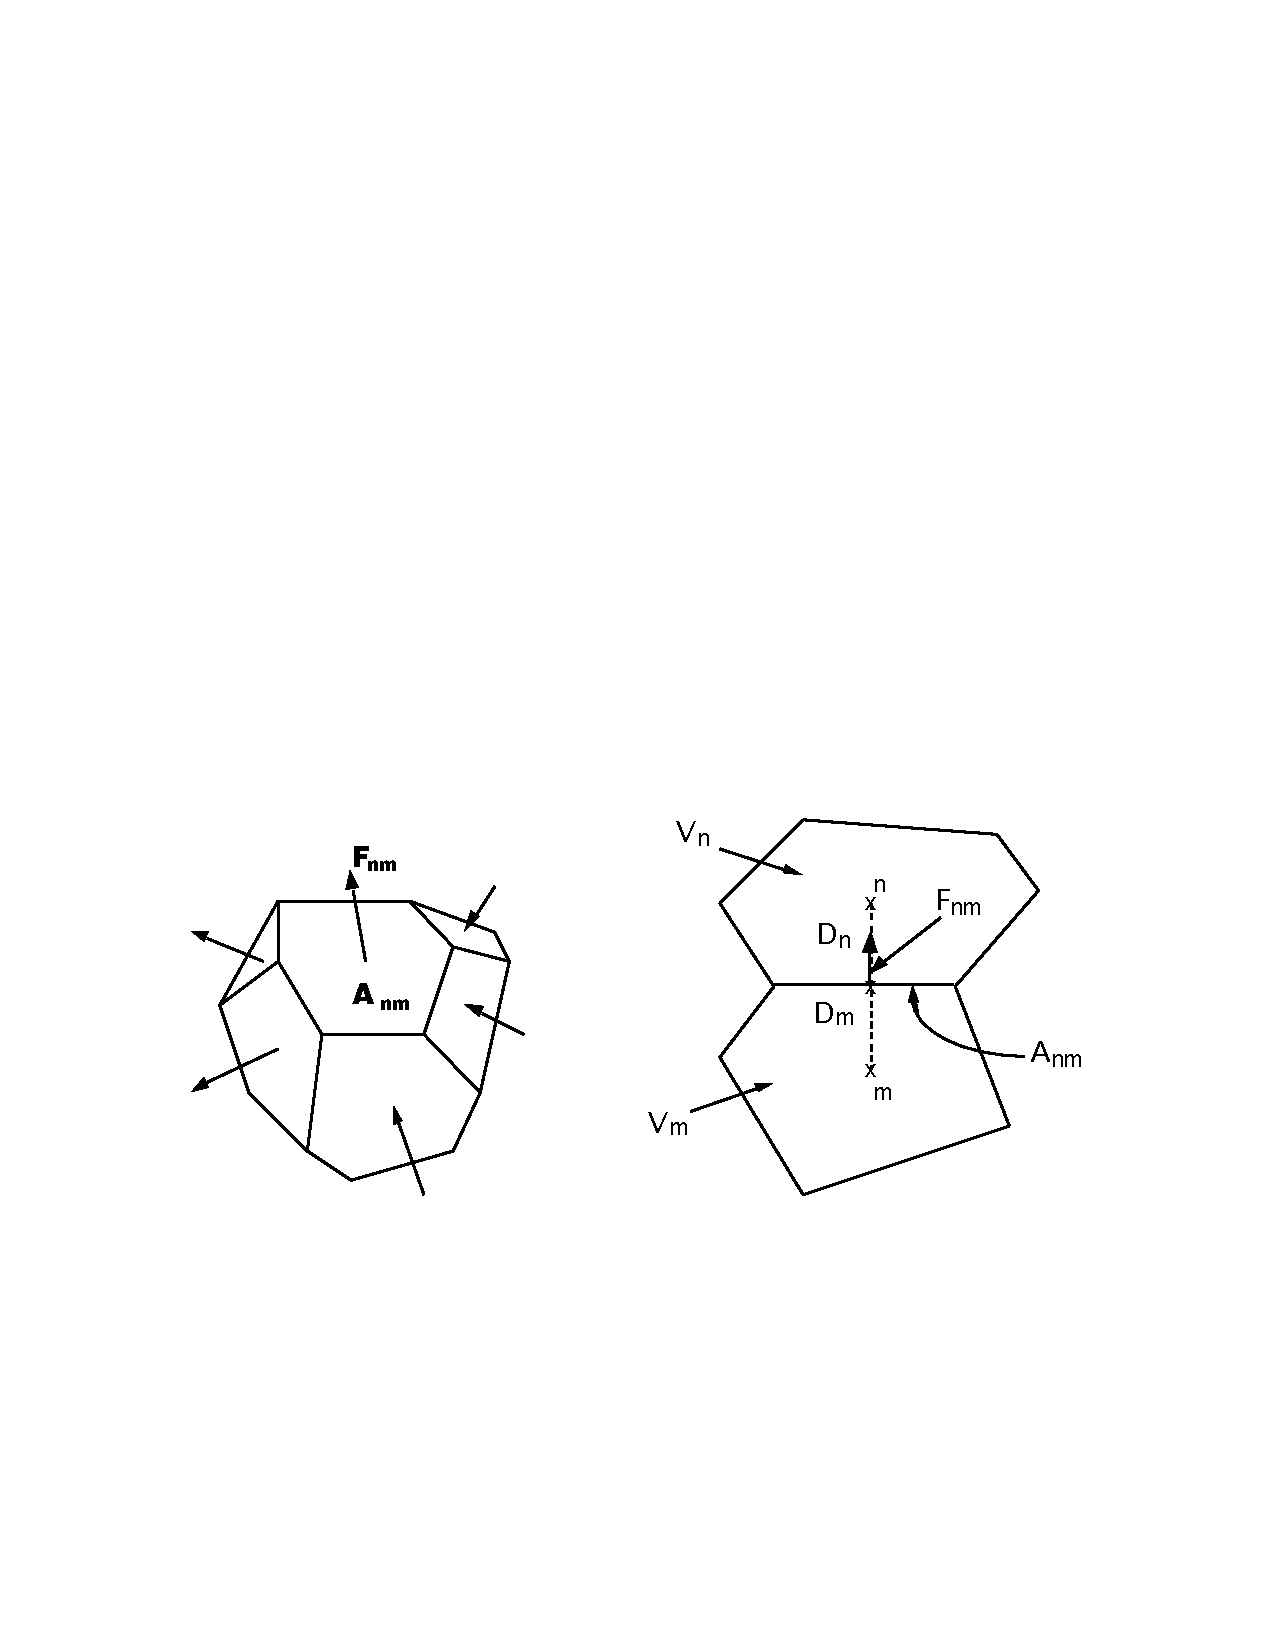
\includegraphics[scale=0.65]{./figs/unstruct_grid}
\caption{General unstructured grid showing control volume, and interfacial areas and fluxes.}\label{funstruct}
\end{figure}

Partitioning the computational domain into a set of finite volumes $V_n$ (see Figure~\ref{funstruct}) and integrating the partial differential equations over each volume yields a discretized form of the mass conservation equations. The following results are obtained:
\EQ
\int_{V_n} \frac{\p}{\p t} A \,dV \simeq \frac{A_n^{t+\Delta t}-A_n^t}{\Delta t} V_n,
\EN
for the accumulation term,
\EQ
\int_{V_n} \S \,dV \simeq \S_n V_n,
\EN
for the source term, and
\EQ
\int_{V_n} \bnabla\cdot \bF \,dV \eq \int_{\p V_n} \bF \cdot \bdS \simeq \sum_{n'} F_{nn'} A_{nn'},
\EN
for the flux term, where $\p V_n$ denotes the surface of $V_n$, and the sum is over the neighboring volumes connected to $V_n$. The flux $F_{nn'}$ across the $n\!-\!n'$ interface connecting volumes $V_n$ and $V_{n'}$ is defined by
\EQ
F_{nn'} \eq (q \rho)_{nn'} X_{nn'} - (\phi D\rho)_{nn'} \frac{X_n-X_{n'}}{d_n+d_{n'}},
\EN
where the subscript $nn'$ indicates that the quantity is evaluated at the interface, and the quantities $d_n$, $d_{n'}$ denote the distances from the centers of the control volumes $V_n$, $V_{n'}$ to the their common interface with interfacial area $A_{nn'}$.
Combining these results gives the residual equation for the discretized form of the partial differential equations
\EQ
R_n \eq \big(A_n^{k+1}-A_n^{k}\big) \frac{V_n}{\Delta t} + \sum_{n'} F_{nn'} A_{nn'} - \S_n V_n,
\EN
where, in general, $R_n$ is a nonlinear function of the independent field variables and superscript $k$ denotes the $k$th time step. These equations may be solved using a Newton-Raphson iteration technique in which the discretized equations are first linearized resulting in the Newton-Raphson equations
\EQ
\sum_{n'} J_{nn'}^i \,\delta x_{n'}^{i+1} \eq -R_n^i,
\EN
for the $i$th iteration, with the Jacobian matrix $J_{nn'}^i$ defined by
\EQ
J_{nn'}^i\eq\frac{\p R_{n}^i}{\p x_{n'}^i}.
\EN
Typically, for solving the flow equations $\delta x_n = \delta p_n$, where $p$ denotes the fluid pressure, whereas for the reactive transport equations $\delta x_n = \delta \ln C_{jn}$, where $C_{jn}$ denotes the concentration of the $j$th chemical species.

An explicit method is used to solve the mineral mass transfer 
equations 
\EQ
\frac{\p\varphi_m}{\p t}\eq\overline V_m I_m,
\EN
given by: 
\EQ\label{phioft}
\phi_m (\br, \, t+\Delta t) \eq \phi_m (\br, \, t) + \Delta t 
\overline V_m I_m (\br, \, t), 
\EN 
with mineral volume fraction $\varphi_m$ and molar volume $\overline V_m$, where the mineral reaction rate $I_m (\br, \, t)$ is taken from the previous time step. 

\paragraph*{Pseudo code illustrating implementation of the IFV method.}

Pseudo is given below for the flow equation
\EQ
\frac{\p}{\p t} \varphi\rho + \bnabla\cdot\rho\bu\eq 0,
\EN
with $\bu$ given by Darcy's law
\EQ
\bu\eq-\frac{\kappa}{\mu}\nabla\big(p-W\rho g z\big),
\EN
with permeability $\kappa$, viscosity $\mu$, molar fluid density $\rho$, formula weight of water $W$, and acceleration of gravity $g$.
\begin{verbatim}
!accumulation term
  do n = 1, grid%nlmax  ! For each local node do...
    ng = grid%nL2G(n)   ! corresponding ghost index
    voldt = porosity_loc_p(ng) * volume_p(n) / grid%dt
    r_p(jn) = (ddensity_loc_p(ng) - density_p(n)) * voldt
  enddo

!flux terms
  do nc = 1, grid%nconn  ! For each interior connection...
    m1 = grid%nd1(nc) ! node indices other either side of face nc
    m2 = grid%nd2(nc)

    n1 = grid%nG2L(m1) ! local node indices
    n2 = grid%nG2L(m2)
    
    dd1 = grid%dist1(nc) ! distances to interface
    dd2 = grid%dist2(nc)
    
    ip1 = grid%iperm1(nc) ! permeability direction
    ip2 = grid%iperm2(nc)
    
    if (ip1 == 1) then
      perm1 = perm_xx_loc_p(m1) ! permeability in x-direction
    else if (ip1 == 2) then
      perm1 = perm_yy_loc_p(m1) ! permeability in y-direction
    else
      perm1 = perm_zz_loc_p(m1) ! permeability in z-direction
    endif
    
    if (ip2 == 1) then
      perm2 = perm_xx_loc_p(m2)
    else if (ip2 == 2) then
      perm2 = perm_yy_loc_p(m2)
    else
      perm2 = perm_zz_loc_p(m2)
    endif
    
    dd = dd1 + dd2
    f1 = dd1/dd
    f2 = dd2/dd
    
    gravity = grid%fmwh2o * grid%gravity * grid%delz(nc)

    D1 = perm1 / viscosity_loc_p(m1)
    D2 = perm2 / viscosity_loc_p(m2)

    D = (D1 * D2) / (dd2*D1 + dd1*D2)

    density_ave = f2 * ddensity_loc_p(m1) + f1* ddensity_loc_p(m2)

    v_darcy = -D * (ppressure_loc_p(m2) - ppressure_loc_p(m1) & 
                - gravity * density_ave)

    q = v_darcy * grid%area(nc)
    flux = density_ave * q
    
      ! Now add the flux contributions for this phase.
      ! Note that fluxes through a downstream face should be added to the
      ! residual component at the cell, while fluxes through an upstream face 
      ! should be subtracted.  (The divergence gives the net OUTFLOW rate per
      ! unit volume.)  Thus, when working with pressure differences,
      ! (ppressure(jm2) - ppressure(jm1)) should be *subtracted* at the 
      ! upstream node n1 because q = -D*div(P).
    
    if (n1 > 0) then  ! If the upstream node is not a ghost node...
      r_p(n1) = r_p(n1) + flux
    endif

    if (n2 > 0) then ! If the downstream node is not a ghost node...
      r_p(n2) = r_p(n2) - flux
    endif
  enddo
  \end{verbatim}

\end{document}
